\documentclass[conference]{IEEEtran}
\IEEEoverridecommandlockouts
% The preceding line is only needed to identify funding in the first footnote. If that is unneeded, please comment it out.
%Template version as of 6/27/2024

\usepackage{cite}
\usepackage{amsmath,amssymb,amsfonts}
\usepackage{algorithmic}
\usepackage{graphicx}
\usepackage{textcomp}
\usepackage{xcolor}
\usepackage[nomarkers,figuresonly]{endfloat}
\renewcommand{\efloatseparator}{\mbox{}}

\def\BibTeX{{\rm B\kern-.05em{\sc i\kern-.025em b}\kern-.08em
    T\kern-.1667em\lower.7ex\hbox{E}\kern-.125emX}}
\begin{document}

\title{Navigating the LLM Surge: AI-Driven Load Balancing}

\author{\IEEEauthorblockN{1\textsuperscript{st} Luis Dale Gascon}
\IEEEauthorblockA{\textit{Department of Computer Science} \\
\textit{Towson University}\\
Towson, United States \\
lgascon1@students.towson.edu}
\and
\IEEEauthorblockN{2\textsuperscript{nd} Brendan George Lauterborn}
\IEEEauthorblockA{\textit{Department of Computer Science} \\
\textit{Towson University}\\
Towson, United States \\
blaute3@students.towson.edu}
}

\maketitle

\begin{abstract}
The widespread adoption of artificial intelligence across diverse applications has accelerated significant breakthroughs in many fields. Critically, the explosion of generative AI and multi-modal Large Language Models (LLMs) has introduced unprecedented network strain, pushing existing infrastructure to its limits. The massive data flows required for LLM training and real-time inference, coupled with low-latency demands for interactive multi-modal chat bots, highlights a growing demand of improving network response times.

In response to this challenge, researchers are exploring different ways load balancers could be improved through AI. Reinforcement learning, for instance, enables AI agents to autonomously learn optimal load distribution strategies. This capability presents a promising alternative to conventional methods, offering the potential for networks to dynamically adapt and scale to meet the fluctuating and intense demands of LLMs. Our current research aggregates the findings from multiple studies to identify commonalities in the challenges, inherent limitations, and achieved outcomes within this evolving domain, aiming to pave the way for more resilient and efficient AI-driven network solutions.
\end{abstract}

\begin{IEEEkeywords}
Reinforcement Learning, Load Balancing, Cloud Computing, AI-driven Load Management, LLM, Supervised Learning, Software Defined Network.
\end{IEEEkeywords}

\section{Introduction}

While traditional web applications often exhibit relatively predictable traffic patterns, the exponential surge in generative AI usage fundamentally alters this landscape. Unlike conventional web traffic workloads, the dynamic, and computationally intensive nature of generative AI applications, especially multi-modal content, renders traditional round-robin or utilization-based traffic management techniques generally unsuited for optimal load distribution \cite{Berenberg_Sambi_2024}.

As generative AI tools and LLMs like GPT, Gemini, CoPilot, and Grok continue their rapid growth and widespread adoption, their associated internet traffic is escalating significantly. With AI now actively assisting across diverse sectors such as education, healthcare, elderly care, and social support, this trend shows no signs of abatement. For instance, OpenAI and ChatGPT alone recorded 551.1 million monthly visitors in September 2024, representing a substantial 22.96\% increase compared to the previous month \cite{Koneva_2025}. This burgeoning popularity directly translates into unprecedented demands on network infrastructure.

Considering the remarkable advancements in artificial intelligence, particularly its demonstrated ability to come up with optimal solutions for complex problems during runtime, it is logical to explore its application in mitigating the challenges of network load balancing. This research posits that AI-driven methodologies can significantly enhance the adaptability and efficiency of network resource management.

We begin in Section II with a foundational overview of key concepts, setting the stage for the detailed analyses that follow. Section III then takes a deep dive into specific case studies, illustrating how machine learning algorithms are being employed to train models with the aim of surpassing traditional load balancing approaches. Concluding this exploration, Section IV identifies and discusses potential avenues for future improvements suggested by these studies.

\section{Background}

\subsection*{Traditional Load Balancing}

Despite the already existing load balancing techniques in SDN, there are still issues with dynamic load balancing. Dynamic methods can help to distribute loads, however they use load balancers’ pre-programmed patterns \cite{Alhilali_Montazerolghaem_2023}. This method is better than static load balancing, but it still relies on fixed patterns that are not truly adaptive to unpredictable conditions.

\subsubsection*{Static Load Balancing}
Distributes load on fixed rules. It lacks real time load consideration during runtime. It is suitable for stateless applications.

\textbf{Round-Robin:} Distributes load sequentially across servers. Although the simplicity of this algorithm is appreciated, this algorithm struggles when resources have unequal capabilities.

\subsubsection*{Dynamic Load Balancing}

Dynamically identifies the amount of load that needs to be distributed during runtime, so it logically selects which servers should bear the load. It is suitable for stateful applications.

\textbf{Least Connections:} Distributes load first to the server with the least amount of active connections during runtime.

\subsection*{Software-Defined Networking (SDN)}
Software Defined Network was introduced to make the network infrastructure more flexible. This design separates the control plane from the data plane and allows for a more flexible, scalable, and cost-effective network architecture\cite{Latah_Toker_2019}. In this design, the data plane represents the bottom layer. The data plane is known as the infrastructure layer and is made up of interconnected forwarding units that forward packets based on rules set by the controller. The control plane represents the intermediate layer and is managed by a centralized SDN controller. The SDN controllers determine the network forwarding behavior.

\subsection*{Q-learning algorithm}

A model-free reinforcement learning technique. Model-free means that the machine learns through trial and error without any knowledge of the environment its being trained on and its constraints. Similar to playing a board game without reading the rule book.

The core idea lies behind a Q-table, a data structure consisting of a set of actions and states where the algorithm updates the value in the table over the course of training.

The Q-learning algorithm used in the case studies (Bellman's Equation) can be summarized with the following equation:
\[
\text{New }Q(s,a) \leftarrow Q(s,a) + \alpha [r + \gamma \; \text{max} \; Q(s\prime, a\prime) - Q(s,a)]
\]

where:

\begin{itemize}
    \item $s$: Current state of the agent
    \item $a$: Action an agent takes
    \item $r$: Reward or the direct feedback
    \item $\gamma$: Discount factor. A low value results in a greedy agent, where it prioritizes short term gains, instead of the long term.
    \item $\alpha$: Learning rate. A hyperparameter of how quickly a model can achieve convergence. 
\end{itemize}

\subsection*{Supervised Learning}

Supervised learning is a subset of machine learning in which a model is trained using data. The dataset contains inputs that are mapped to corresponding outputs. By learning these relationships, the model can make accurate predictions for any future data.


\section{Use of Machine Learning for Load Balancing}

\subsubsection*{Case Study: Optimizing SDN Controller Placement}\label{AA}
Mu He introduced a multi-label classification approach to predict global network allocations \cite{He_Kalmbach_Blenk_Kellerer_Schmid_2017}. That is, each network node can be linked to multiple controllers, allowing the nodes to be partially controlled by more than one controller. Each link has a weight. Due to the weight of the links, it allows the load to be more flexible. The Neural Network is trained to learn the relationship between the input and output. The input is the current traffic distribution in the network and the output being the optimal controller locations for that traffic. See Fig. \ref{fig:heuristic} for a high level diagram of the process.

\textbf{Decision Trees}
Decision trees can also use multi-label classification by employing the binary relevance approach \cite{He_Kalmbach_Blenk_Kellerer_Schmid_2017}. This builds separate trees that are trained independently. Simple if/then rules are applied to split the data based on feature values. The outputs are combined in the end to predict controller placement or path selection. However, each tree is built and trained independently of each other and cannot capture nonlinear relationships.

\textbf{Logistic Regression}
Logistic Regression is similar to Decision Trees in that it predicts whether a controller is placed on each node \cite{He_Kalmbach_Blenk_Kellerer_Schmid_2017}. LR takes weighted inputs such as bandwidth, latency and packet loss and calculates a weighted sum of these inputs. The Sigmoid Function is then applied which assigns each node a value between 0 and 1, which represents the probability that node is assigned a controller. From there, a decision is made based on a certain threshold. Logistic Regression is limited to modeling linear relationships between the input and output.

\textbf{Neural Network}
The Neural Network goes a step further than the Logistic Regression. Inputs such as bandwidth, latency and packet loss undergo a series of nonlinear transformations, as they move through hidden layers of the network. The hidden layer is made up of nodes that apply weighted sums and an activation function to capture relationships from the data. After these transformations, the output is passed to the output layer, which produces the final prediction. Neural Networks learn label correlations and nonlinear patterns in the traffic data. Mu He describes that the Neural Network adjusts its weights during the training using the Bernoulli Cross Entropy loss and the ADAM optimizer to reduce prediction errors. As a result of these improvements, Neural Network is more effective for dynamic controller placement in Software Defined Networks. We discuss an example of a Neural Network, known as the Back Propagation Artificical Neural Network, later in this paper. 

\textbf{Results and Summary}
In the case study, Mu He finds that NN-LS, a combination of Neural Network and Local Search, reduces the algorithm runtime by two thirds. This is a significant increase in efficiency and shows positive results that motivate further research to be done around AI’s impact on networks. However, finding the ideal solution is not that easy. There are multiple network topologies that exist in the real world. Mu He tests the three machine learning  techniques, DT, LS and NN for BICS and Cogentco to determine how well they place controllers. He demonstrates that NN and LS perform well for BICS. DT does not perform as well in this given network topology. However, for Cogentco, DT performs better than LS and NN. As more controllers are added, the differences between DT and the other two get larger. We conclude that it is difficult to make an exact prediction of controller placement. There is not a single correct algorithm that wins in every scenario. Nevertheless, the use of AI techniques shows promise for making controller placement more efficient. Having better controller placement will reduce latency and balance traffic. 

\subsubsection*{Case Study: Decreasing Network Latency with Neural Networks }

Cui Chen-Xiao an Xu Ya-Bin performed research on load balance in Software Defined Network. Four load features are introduced to help determine the most optimal transmission path. These features are bandwidth utilization ratio, packet loss rate, transmission latency and transmission hops\cite{Chen-Xiao_Ya-bin_2016}. A Backpropagation artificial neural network model is also introduced and trained using these four features. The goal of this model is to predict the integrated load for each path and select the most optimal one.


The artificial neural network computing model is very powerful because it is nonlinear, self-learning, and has no limit on input vectors. Therefore, it can capture very complex relationships and handle unpredictable datasets. This is critical for Software Defined Networks because traditional load balancing methods are limited and can be improved. In the following sections, we discuss the 3-layer Back Propagation Artificial Neural Network. The BPANN is a specific type of Artificial Neural Network that is introduced by Chen-Xiao and Ya-Bin. The BPANN has two main phases.

\textbf{Forward Propagation Learning Phase}
The Forward Propagation Learning phase is designed to pass input data through the model and make a prediction. A 3-layer BPANN consists of an input layer, a hidden layer, and an output layer. The input layer is the starting point for the learning phase. This layer passes the raw data forward to the hidden layer. The input neurons process the input data known as input vectors. Each input is multiplied by preset weights through the action function\cite{Chen-Xiao_Ya-bin_2016}. The output of the hidden layer is then passed to the output layer where it applies its own weights and activation actions. The output layer then outputs the ultimate results. After the learning phase, the BPANNN will enter the weight adjustment phase.

\textbf{Weighted Adjustment Phase}
The goal of the weight adjustment phase is to adjust the weights in the hidden and output layers to improve accuracy. This is achieved by comparing the ultimate results from the forward propagation learning phase with the expected results to calculate the error. The network will then use this error to adjust the neuron weights accordingly. The model propagates the weight adjustments backward through the network starting with the output layer. The model will repeat the forward and backward process until the error meets the standards. By training the model, the BPANN will eventually find the most optimal weight for the given case. These two phases allow the BPANN to learn from the data and adapt to network conditions.

\textbf{Application of BPANN}
Now that we have learned how the BPANN model operates, we discuss the research conducted by Chenxiao and Yabin. The authors were able to train the BPANN to predict path load conditions. Thus, allowing the system to properly select the transmission path and balance the network traffic. This research helps us understand the benefits of using Artificial Intelligence to balance loads more efficiently compared to static methods. 

\textbf{Experimental Setup}
In the experiment, Chen-Xiao and Ya-Bin simulate a multipath SDN environment using the Mininet Network Simulation tool and Floodlight SDN Controller. The path load features are recorded by the SDN controller using OpenFlow This setup allows them to monitor network performance. To mimic real-world scenarios, the experiment utilizes multiple hosts (Hosts 2-7) that send traffic to each other randomly. Thus, simulating different loads on different paths. Once the network traffic is busy, Host 1 sends traffic to Host 7. This new data flow needs to pick a path through the network with the lightest load. The purpose of this simulation is to avoid congestion among the new path and achieve load balance. The model must be trained using this network traffic data.

\textbf{Training the BPANN}
To minimize prediction error, the model is trained using data from the mininet simulation. The random traffic and load features were collected over 180 second intervals. The BPANN was also trained using different numbers of neurons in the hidden layer. The model was trained having the number of neurons set at 3, 5, 7, 9 and 11.

\textbf{Results and Summary}
Evenly distributing loads in Software Defined Networks remains to be one of the biggest challenges due to the unpredictability of traffic. This experiment demonstrates the ability to leverage Artificial Intelligence to adapt to real-time path load conditions by collecting bandwidth utilization ratio, packet loss rate, transmission latency and transmission hops. By introducing and testing the BPANN, the authors find that this model provides better network performance and can decrease network latency up to 19.3\% \cite{Chen-Xiao_Ya-bin_2016}. These results prove that the use of Artificial Intelligence allows more flexibility and improves load management in Software Defined Networks.

\subsection{Reinforcement Learning}

Reinforcement Learning (RL) provides models with the ability to learn adaptively from continuous interactions with their environment, making decisions based on accumulated experiences until it converges to an ``optimal'' behavior through indicators. This offers a distinct advantage over supervised learning, where models are trained solely on labeled datasets and thus lack the capacity to evolve and continuously improve with real-time network adjustments.

\subsubsection*{Case Study: Agentic AI}

A Reinforcement Learning Agent monitors real-time metrics such as response time, task completion rate and server utilization. It uses those metrics to make dynamic decisions regarding which server should handle each task.

\textbf{Experimental Setup} A simulated cloud environment was constructed with CloudSim, a toolkit for simulating cloud computing infrastructures. Within this environment, a dedicated task scheduler component was implemented to receive and manage incoming workload requests, serving as the interface for providing real-time operational data to the Artificial Intelligence (AI) agent currently undergoing training. Reinforcement learning was implemented in Python with Numpy and OpenAI Gym, now called Gymnasium, libraries.

The simulated cloud infrastructure comprised a heterogeneous pool of ten virtual machines (VMs), each configured with varying computational capacities to accurately reflect real-world diversity. The core mechanism involved the AI agent's objective to assign these tasks to the available VMs, with the efficacy of its assignments reflected in the reward function of the reinforcement learning process; improvements in network performance metrics, such as reduced response times, and lower resource utilization on individual VMs were designed to yield higher positive rewards, allowing the AI agent to iteratively refine its load balancing strategy.\cite{Kavish_Chawla_2024}

\textbf{Results and Summary}

The AI agent's performance significantly outperforms traditional load balancing methods in all of the performance metrics. The traditional load balancing methods compared with are round-robin, least connections and weighted load balancing.

See Fig \ref{fig:response} and \ref{fig:utilization} for the visual results.

\textbf{Future Improvements and Limitations}
While the computational cost of training a model to yield an optimal output costs a more than exponential relationship with the scale of its environment, the significant upfront investment is offset by its subsequent efficiency; once trained, the model demonstrates its ability to work with traffic changes with negligible additional overhead. Nevertheless, a crucial avenue for further improvement involves bolstering the model's capacity for seamless adaptation within extremely heterogeneous cloud environments, a common characteristic of contemporary cloud infrastructures.

\section{Conclusion}

The various case studies underscore the potential of novel machine learning techniques to fundamentally improve load balancing. This is particularly relevant given that the flourishing demand for agentic AI and its multi-modal capabilities has introduced unprecedented strain on both computational resources and network performance. While supervised learning techniques, as demonstrated in earlier research, offer a valuable means of anticipating future traffic based on historical patterns, reinforcement learning, specifically utilizing the Q-learning algorithm, introduces a highly promising avenue for dynamic, runtime optimization of load balancing processes.

\begin{figure}
    \centering
    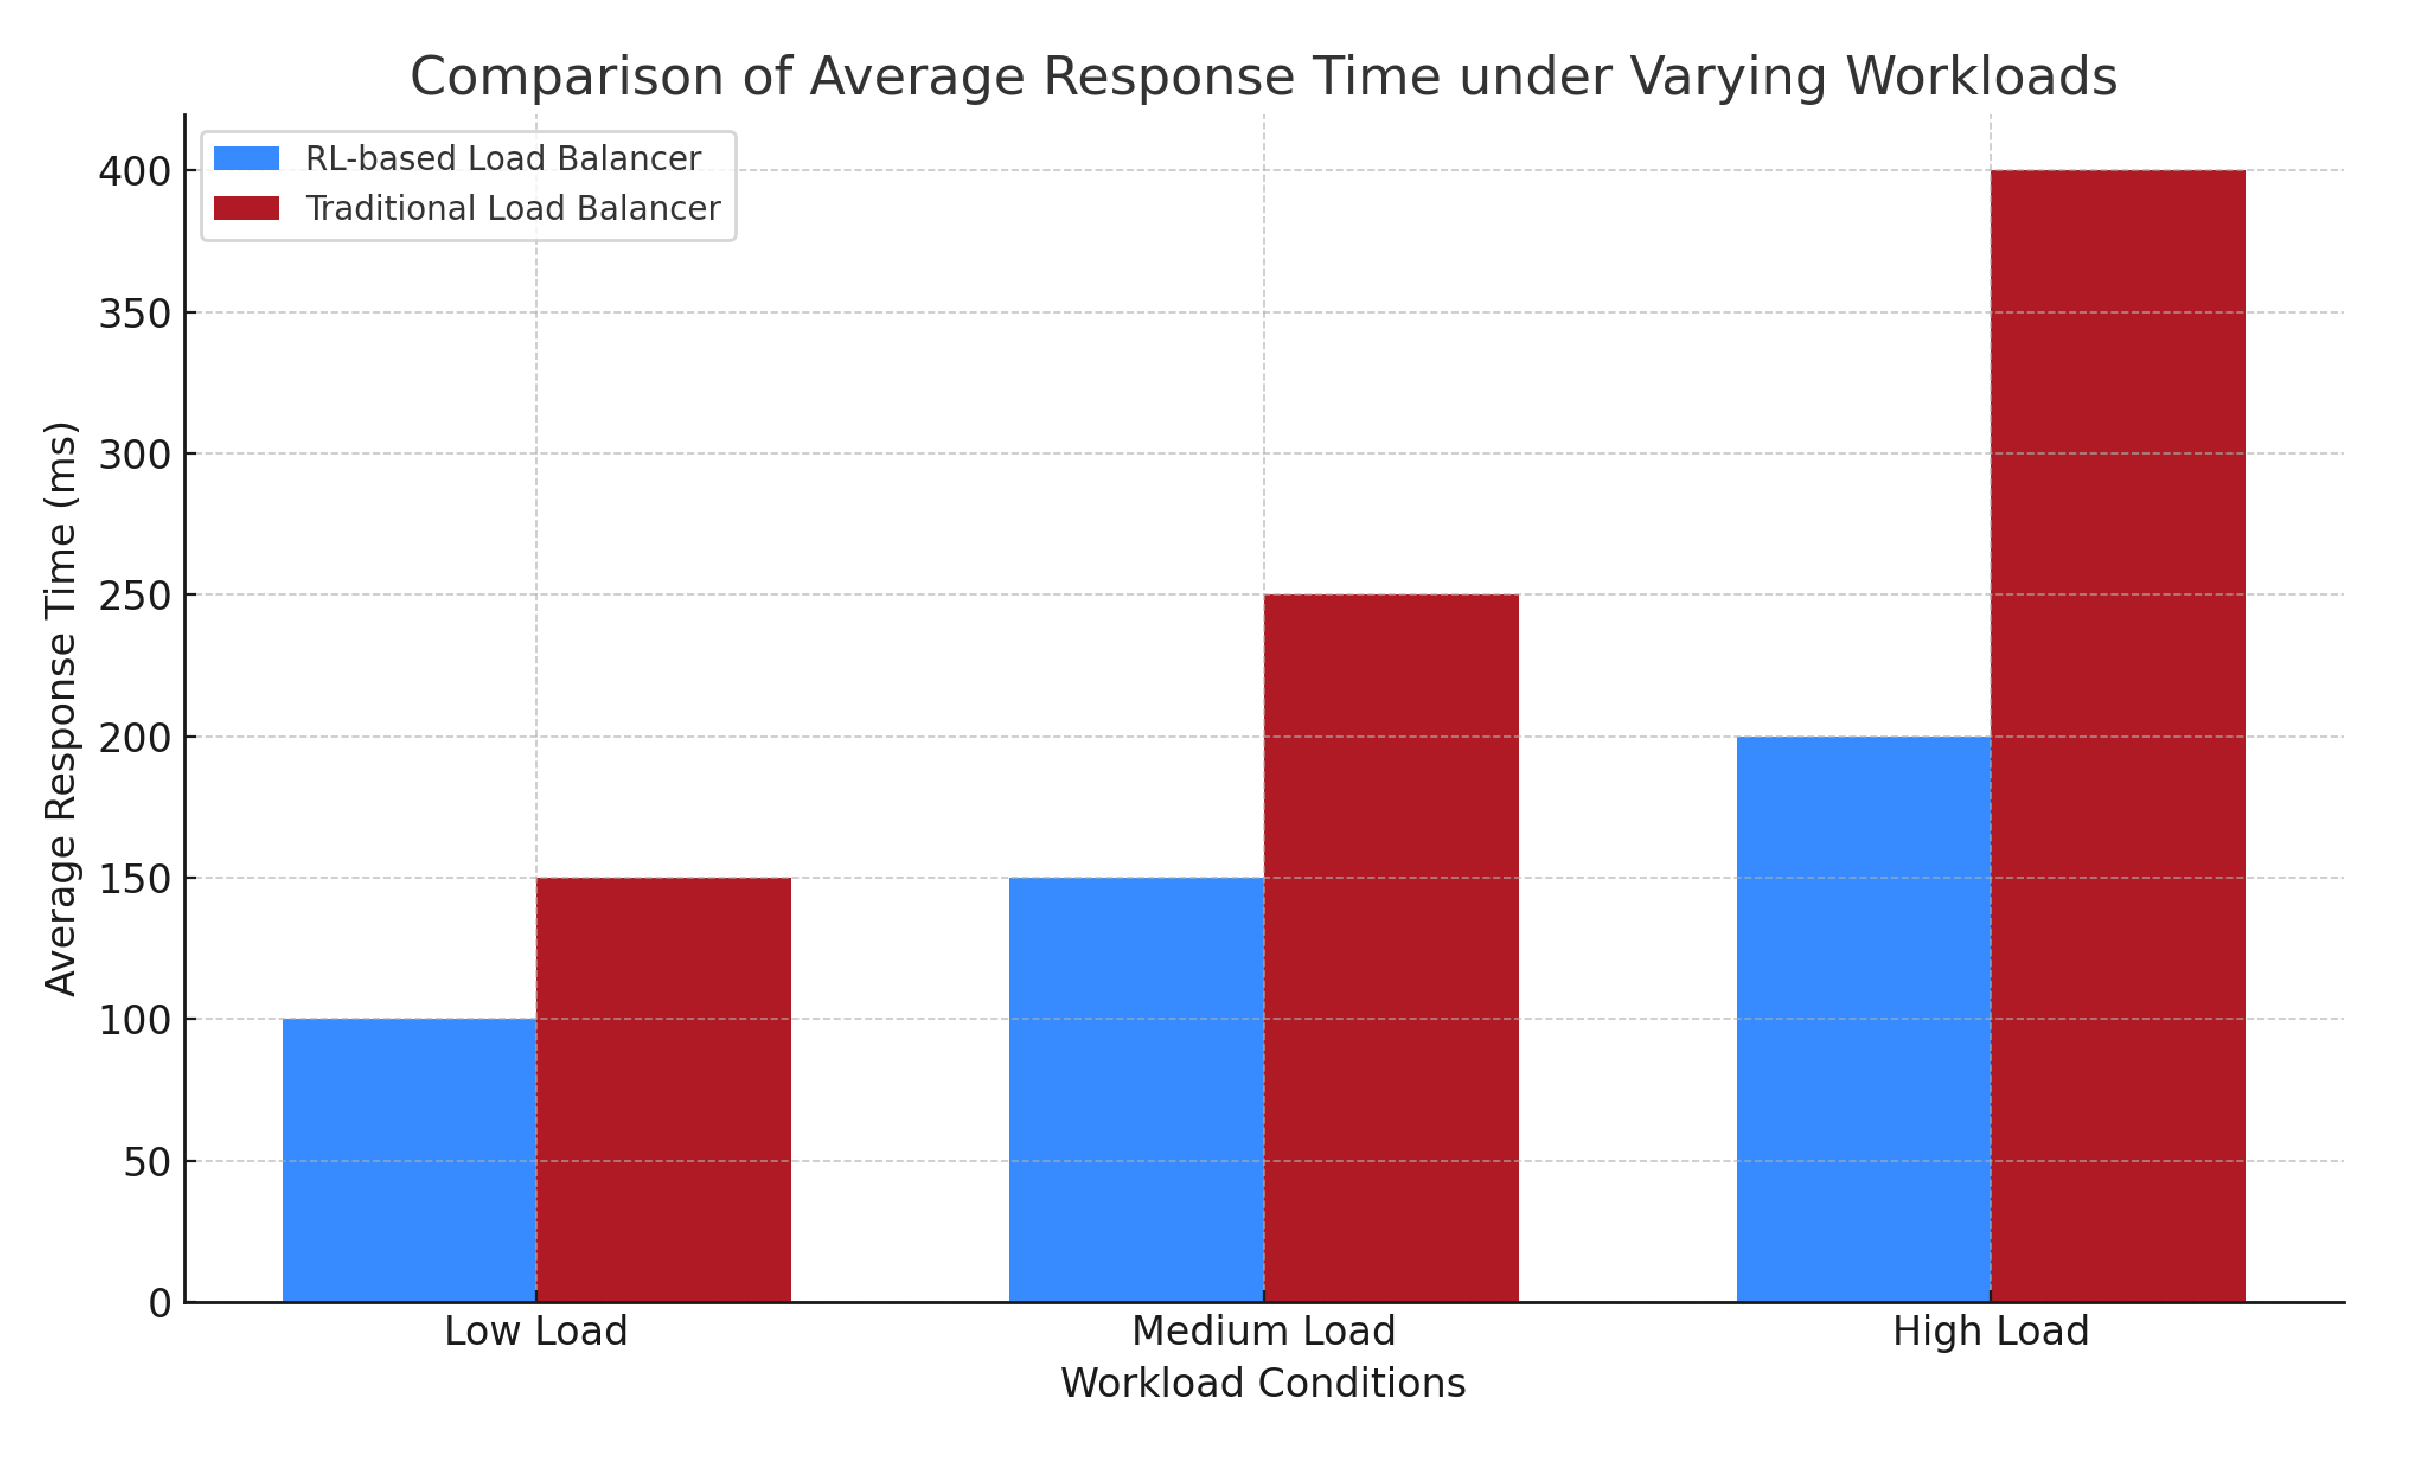
\includegraphics[width=.5\linewidth]{response_time.png}
    \caption{Average response time comparison between traditional and AI-driven load balancers}
    \label{fig:response}
\end{figure}

\begin{figure}
    \centering
    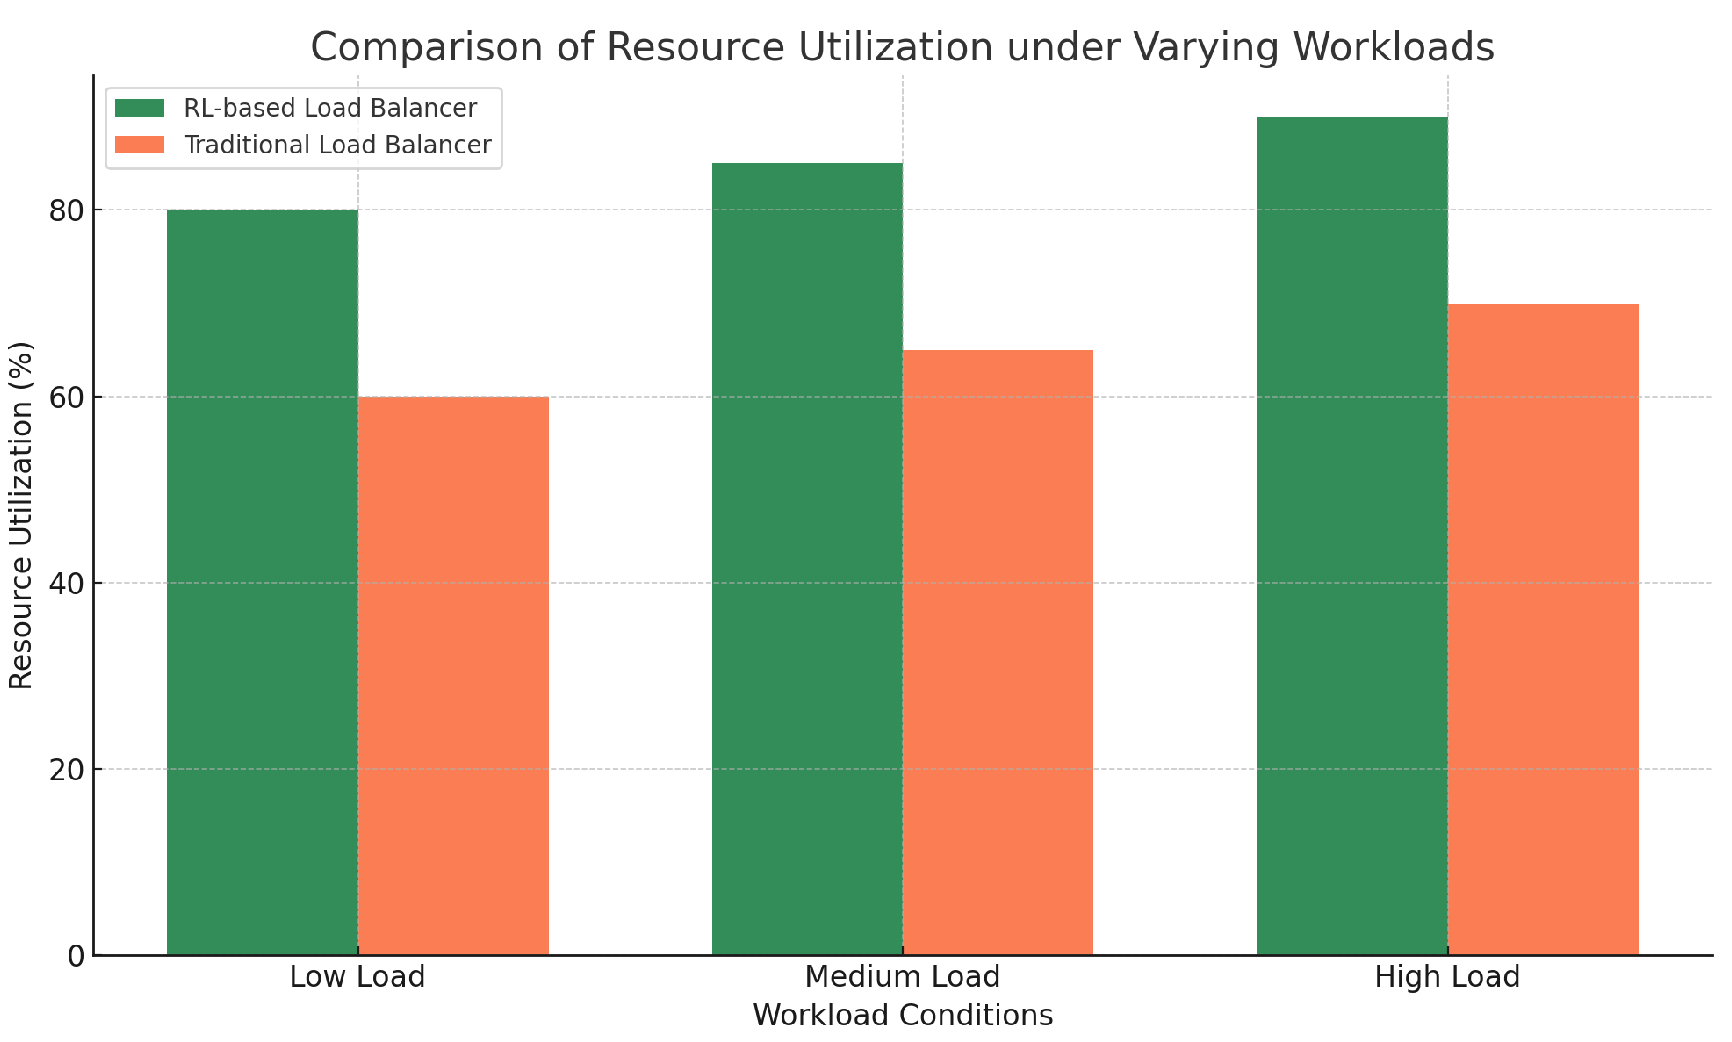
\includegraphics[width=.5\linewidth]{resource_utilization.png}
    \caption{Resource Utilization comparison between traditional and AI-driven load balancers}
    \label{fig:utilization}
\end{figure}

\begin{figure}
    \centering
    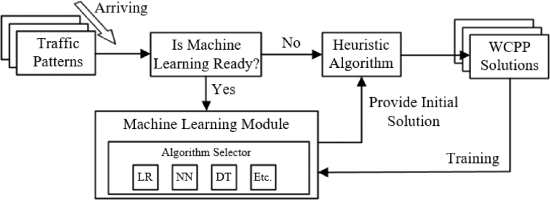
\includegraphics[width=.5\linewidth]{heuristics.png}
    \caption{Heuristic Algorithm using trained models}
    \label{fig:heuristic}
\end{figure}

\bibliographystyle{IEEEtran}
\bibliography{ref}

\end{document}
